\section{Frank-Wolfe Algorithm}

This is to solve constrained optimization, similar to PGD.

\textbf{Definitions}:
\begin{enumerate}
    \item \textbf{Linear minimization oracle (LMO)}: $\LMO_X(g) = \argmin_{z\in X} g^\top z$.
    \item \textbf{Frank-Wolfe algorithm}: do $s = \LMO_X(\nabla f(x_t))$ and $x_{t+1} = (1-\gamma_t)x_t+\gamma_t s$. Benefits: (1) the iterates are always feasible for convex domain; (2) the algorithm is projection-free if we can solve LMO; (3) the iterates have a sparse representation, defined by the combination of LMO in the previous steps; (4) it is affine-invariant, meaning that affine equivalent problems can be solved at the same cost, i.e., if $g(x)=f(Ax+b)$ and $\dom(g)=A^{-1}(\dom(f)-b)$, then minimizing $g$ is the same to minimizing $f$.
    \item \textbf{Curvature constant}: the curvature constant of the constrained optimization is defined to be $C_{f,X} = \sup_{y=(1-\gamma)x+\gamma s, \gamma \in (0,1]} \frac{1}{\gamma^2} (f(y) - f(x) - \nabla f(x)^\top (y-x))$. 
\end{enumerate}

\textbf{LASSO ($L_1$ domain)}: minimize $\|Ax-b\|^2$ subject to $\|x\|_1\le 1$. Thus, $\LMO_X(g) = \argmin_{z = \pm e_i, i\in [n]} g^\top z = -\sgn(g_i) e_i$, where $i = \argmax |g_i|$. Therefore, we can compute LMO in $O(\log(d))$.

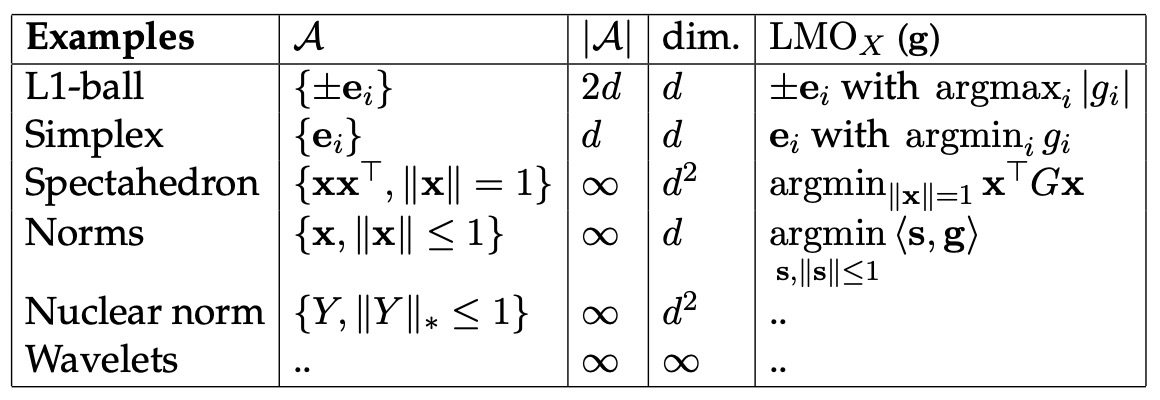
\includegraphics[width=\linewidth]{imgs/LMO.jpg}

\textbf{Duality gap as a certificate for optimization quality}: We define the duality gap at $x$ to be $g(x) = \nabla f(x)^\top (x-s)$, where $s = \LMO_X(\nabla f(x))$. (8.2) For convex $f$, $g(x) \ge f(x) - f(x^*)$. Proof: $g(x) = \nabla f(x)^\top x - \min_{z \in X} \nabla f(x)^\top z \ge \nabla f(x)^\top x - \nabla f(x)^\top x^* \ge f(x) - f(x^*)$.

\textbf{Analysis}:
\begin{enumerate}
    \item \textbf{Decrease property}: (8.4) for $\gamma_t \in [0,1]$, we have $f(x_{t+1}) \le f(x_t) - \gamma_t g(x_t) + \gamma_t^2 \frac{L}{2}\|s-x_t\|^2$, where $g(x_t)$ is the duality gap. Proof: by smoothness, $f(x_{t+1}) \le f(x_t) + \nabla f(x_t)^\top \gamma_t(s-x_t) + \gamma_t^2 \frac{L}{2}\|s-x_t\|^2 = f(x_t) - \gamma_t g(x_t) + \gamma_t^2 \frac{L}{2}\|s-x_t\|^2$.
    \item \textbf{Affine-invariant decrease}: we have $f(x_{t+1}) \le f(x_t) - \gamma_t g(x_t) + \gamma_t^2 C_{f,X}$. Proof: plug in $x=x_t$, $y=(1-\gamma_t)x_t+\gamma_t s$ into the definition of curvature constant.
    \item $\gamma_t = \frac{2}{t+2}$: (8.3) assume $f$ is convex and $L$-smooth, and $X$ is convex, closed and bounded, then $f(x_T) - f(x^*) \le \frac{2LR^2}{T+1}$, where $R = \max_{x,y\in X}\|x-y\|$. Proof: define $h(x) = f(x) - f(x^*)$, thus $h(x_{t+1}) \le h(x_t) - \gamma_t h(x_t) + \gamma_t^2 \frac{L}{2}\|s-x_t\|^2 \le (1-\gamma_t)h(x_t) + \gamma_t^2 C$, where $C = \frac{L}{2}R^2$. By induction, we have $h(x_t) \le \frac{4C}{t+1}$. (8.5) The same holds for $C_{f,X}$ instead of $C$.
    \item $\gamma_t^\prime = \argmin_{\gamma \in [0,1]} f((1-\gamma)x_t + \gamma s)$: the same result holds as now we have $h(x_{t+1}) \le h((1-\gamma_t)x_t + \gamma_t s) \le (1-\gamma_t)h(x_t) + \gamma_t^2 C$.
    \item $\gamma_t^\prime = \min(\frac{g(x_t)}{L\|s-x_t\|^2}, 1)$: the same result holds as now we have $h(x_{t+1}) \le h(x_t) - \gamma_t g(x_t) + \gamma_t^2 C$ as well, since $\gamma_t^\prime$ minimizes this upper bound.
    \item \textbf{Convergence of duality gap}: (8.7) under the same setting, $g(x_t) \le O(\frac{C_{f,X}}{T+1})$.
\end{enumerate}